% #############################################################################
% This is Chapter 1
% !TEX root = ../main.tex
% #############################################################################
% Change the Name of the Chapter i the following line
\chapter{Introduction}
\chaptoc
% The following line allows to ref this chapter
\label{chap:intro}
\noindent \todo[color=green!40,author=Rui Cruz, inline]{The examples of techniques, tools, and packages along the document are for you to get familiarized with them. It is advisable to preserve those examples of usage, for reference, by moving the respective blocks of text to the last Chapter of this template (or to a Chapter file that you know you will not use), until you finish your document.}

\textcolor{violet}{Example of using package} \verb:todo: \textcolor{violet}{for notes of authors.} \textcolor{violet}{In this case} \todo[color=yellow!40,author=Johnny, fancyline]{pointing out to the place} \textcolor{violet}{the author Johnny is calling the attention for something at the specific place in the text.}

\textcolor{violet}{In this other case, another co-author is commenting on something inline.} \todo[color=orange!40,author=Manuel, inline]{Inline comment or Note. It can be an extract of some recommended text. ``Lorem ipsum dolor sit amet, consectetuer adipiscing elit. Morbi commodo, ipsum sed pharetra gravida, orci magna rhoncus neque, id pulvinar odio lorem non turpis. Nullam sit amet enim. Suspendisse id velit vitae ligula volutpat condimentum. Aliquam erat volutpat. Sed quis velit. Nulla facilisi. Nulla libero. Vivamus pharetra posuere sapien.''}

\textcolor{violet}{In this other case, another co-author is making a note about the citation for missing some bibliographic record}~\cite{Apple:2011fk,AdobeHDS:ys,A.:qy}.
\todo[color=red!40,author=Pete]{You should cite also Pellentesque:2014}


Nam consectetuer. Sed aliquam, nunc eget euismod ullamcorper, lectus nunc ullamcorper orci, fermentum bibendum enim nibh eget ipsum. Donec porttitor ligula eu dolor. Maecenas vitae nulla consequat libero cursus venenatis. Nam magna enim, accumsan eu, blandit sed, blandit a, eros.

Quisque facilisis erat a dui. Nam malesuada ornare dolor. \enquote{Cras gravida, diam sit amet rhoncus ornare, erat elit consectetuer erat, id egestas pede nibh eget odio.}\todo[color=green!40,author=Rui Cruz, fancyline]{notice here how to enquote correctly}{} 

Proin tincidunt, velit vel porta elementum, magna diam molestie sapien, non aliquet massa pede eu diam. Aliquam iaculis. Fusce et ipsum et nulla tristique facilisis. Donec eget sem sit amet ligula viverra gravida. Etiam vehicula urna vel turpis. Suspendisse sagittis ante a urna. Morbi a est quis orci consequat rutrum. Nullam egestas feugiat felis. Integer adipiscing semper ligula. Nunc molestie, nisl sit amet cursus convallis, sapien lectus pretium metus, vitae pretium enim wisi id lectus. Donec vestibulum. Etiam vel nibh. Nulla facilisi. Mauris pharetra. Donec augue. Fusce ultrices, neque id dignissim ultrices, tellus mauris dictum elit, vel lacinia enim metus eu nunc.

\textcolor{violet}{This is an example of Tracking} \replaced[id=JO]{Changes}{Xanges} (in this case a replacement) by different authors in the document. The Text can additionally be modified by \added[id=PT]{adding} new text or by deleting \deleted[id=MN]{wrong} inadequate text. Author can manipulate changes \replaced[id=PT]{introduced by each author\deleted[id=MN]{, as adequate}}{intrroduced by other authors}.

Proin at eros non eros adipiscing mollis. Donec semper turpis sed diam. Sed consequat ligula nec tortor. Integer eget sem. Ut vitae enim eu est vehicula gravida. Morbi ipsum ipsum, porta nec, tempor id, auctor vitae, purus. Pellentesque neque. Nulla luctus erat vitae libero. Integer nec enim. Phasellus aliquam enim et tortor. Quisque aliquet, quam elementum condimentum feugiat, tellus odio consectetuer wisi, vel nonummy sem neque in elit. Curabitur eleifend wisi iaculis ipsum.
% #############################################################################
\section{Morbi ipsum ipsum}
Pellentesque nibh felis, eleifend id, commodo in, interdum vitae, leo. 
 Praesent mauris \ac{SD} and \ac{HD} volutpat ligula eget enim \acp{WLAN} and 3G\slash 4G \acp{WWAN}.\todo[color=cyan!40, author=RC]{use of ACRONYMS that are defined in file ``Chapters/Thesis-MSc-Aconyms.tex''}

Praesent eu elit. Ut eu ligula. Class aptent taciti sociosqu ad litora torquent per conubia nostra, per inceptos hymenaeos. Maecenas elementum augue nec nisl. Proin auctor lorem at nibh. Curabitur nulla purus, feugiat id, elementum in, lobortis quis, pede. Vivamus sodales adipiscing sapien. Vestibulum posuere nulla eget wisi. Integer volutpat ligula eget enim. Suspendisse vitae arcu. Quisque pellentesque. Nullam consequat, sem vitae rhoncus tristique, mauris nulla fermentum est, bibendum ullamcorper sapien magna et quam. Sed dapibus vehicula odio. Proin bibendum gravida nisl. Fusce lorem. Phasellus sagittis, nulla in hendrerit laoreet, libero lacus feugiat urna, eget hendrerit pede magna vitae lorem. 
 
Aliquam erat \ac{WLAN} volutpat \ac{CPU} mauris nulla fermentum est \ac{OS} Fusce magna mi, porttitor quis, convallis eget, sodales ac, urna.
Pellentesque nibh felis, eleifend id, commodo in, interdum vitae, leo. Praesent eu elit. Ut eu ligula. Class aptent taciti sociosqu ad litora torquent per conubia nostra, per inceptos hymenaeos. Maecenas elementum augue nec nisl. Please notice the use of automatic referencig to objects such as Figures, Tables, equations, Algorithms, sections of a document, etc. by using the command \verb:\Cref{ref}: as in this case pointing to \Cref{fig:cashed}.\todo[color=cyan!40, author=RC, fancyline]{the correct Name of the float object, in this case a Figure, is determined by the system}

\begin{figure}[h]
\centering
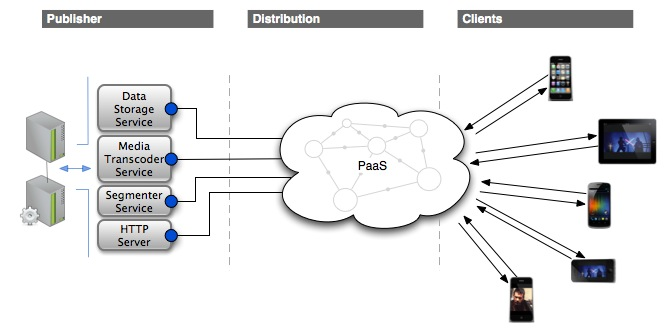
\includegraphics[width=0.9\textwidth]{./Images/cashed5}
\caption{Ecosystem}
\label{fig:cashed}
\end{figure}

Proin auctor lorem at nibh. Curabitur nulla purus, feugiat id, elementum in, lobortis quis, pede. Vivamus sodales adipiscing sapien. Vestibulum posuere nulla eget wisi. Integer volutpat ligula eget enim. Suspendisse vitae arcu. Quisque pellentesque. Nullam consequat, sem vitae rhoncus tristique, mauris nulla fermentum est, bibendum ullamcorper sapien magna et quam. Sed dapibus vehicula odio. Proin bibendum gravida nisl. Fusce lorem. Phasellus sagittis, nulla in hendrerit laoreet, libero lacus feugiat urna, eget hendrerit pede magna vitae lorem. Praesent mauris Class aptent taciti sociosqu ad litora torquent per conubia nostra, per inceptos hymenaeos H.264\slash \ac{AVC} standard, sem vitae rhoncus tristique \ac{SVC} \cite{Fraunhofer-Heinrich-Hertz-Institute:2013fk,ISO:H-264} nulla in hendrerit laoreet, libero lacus feugiat urna, eget hendrerit pede magna vitae lorem.

\textcolor{violet}{You can use in-paragraph lists with this construct for: 
\begin{inparaenum}[(a)]
\item first case;
\item second case; and
\item third case,
\end{inparaenum}
making the text organized and fluid.}

Vivamus auctor leo vel dui. Aliquam erat volutpat. Phasellus nibh. Vestibulum ante ipsum primis in faucibus orci luctus et ultrices posuere cubilia Curae; Cras tempor. Morbi egestas, urna non consequat tempus, nunc arcu mollis enim, eu aliquam erat nulla non nibh. Duis consectetuer malesuada velit. Nam ante nulla, interdum vel, tristique ac, condimentum non, tellus. Proin ornare feugiat nisl. Suspendisse dolor nisl, ultrices at, eleifend vel, consequat at, dolor, morbi egestas, urna non consequat tempus, nunc arcu mollis enim, eu aliquam erat nulla non nibh.

Notice that \gls{maths} makes extensive use of \Glspl{formula}\todo[color=cyan!40, author=RC, fancyline]{example of use of Glossaries}{} which are particularly well rendered in documents produced with \gls{LaTeX}.

Maecenas elementum augue nec nisl. Proin auctor lorem at nibh. Curabitur nulla purus, feugiat id, elementum in, lobortis quis, pede. Vivamus sodales adipiscing sapien. Vestibulum posuere nulla eget wisi. Integer volutpat ligula eget enim. Suspendisse vitae arcu. Quisque pellentesque.
% #############################################################################
\section{Organization of the Document}
This thesis is is organized as follows: \Cref{chap:intro} \todo[color=cyan!40, author=RC, fancyline]{references to doc sections/chapters are automatic}{}interdum vel, tristique ac, condimentum non, tellus. 
In \cref{chap:back} curabitur nulla purus, feugiat id, elementum in, lobortis quis, pede.
In \cref{chap:architecture} consequat ligula nec tortor. Integer eget sem. Ut vitae enim eu est vehicula gravida.
\Cref{chap:implement} morbi egestas, urna non consequat tempus, nunc arcu mollis enim, eu aliquam erat nulla non nibh in \cref{chap:evaluation}.
\Cref{chap:conclusion} suspendisse dolor nisl, ultrices at, eleifend vel, consequat at, dolor.